\documentclass[crop, tikz]{standalone}
\usepackage{tikz}

\usetikzlibrary{arrows,decorations.pathmorphing,backgrounds,positioning,fit,petri, decorations.pathreplacing,shadows,calc}

\definecolor{echoreg}{HTML}{2cb1e1}
\definecolor{sublimedg}{HTML}{171813}
\definecolor{lgry}{HTML}{aaaaaa}
\definecolor{mymauve}{rgb}{0.58,0,0.82}

\tikzset{%
  cascaded/.style = {%
    general shadow = {%
      shadow scale = 1,
      shadow xshift = -2ex,
      shadow yshift = 2ex,
      draw=black,
      thick,
      fill = white},
    general shadow = {%
      shadow scale = 1,
      shadow xshift = -1.5ex,
      shadow yshift = 1.5ex,
      draw=black,
      thick,
      fill = white},
    general shadow = {%
      shadow scale = 1,
      shadow xshift = -1ex,
      shadow yshift = 1ex,
      draw=black,
      thick,
      fill = white},
    general shadow = {%
      shadow scale = 1,
      shadow xshift = -.5ex,
      shadow yshift = .5ex,
      draw=black,
      thick,
      fill = white},
    fill = white, 
    draw,
    thick}}
    
\tikzset{%
  cascadedd/.style = {%
    general shadow = {%
      shadow scale = 1,
      shadow xshift = -4.5ex,
      shadow yshift = 4.5ex,
      draw=black,
      thick,
      fill = white},
    general shadow = {%
      shadow scale = 1,
      shadow xshift = -4ex,
      shadow yshift = 4ex,
      draw=black,
      thick,
      fill = white},
    general shadow = {%
      shadow scale = 1,
      shadow xshift = -3.5ex,
      shadow yshift = 3.5ex,
      draw=black,
      thick,
      fill = white},
    general shadow = {%
      shadow scale = 1,
      shadow xshift = -3ex,
      shadow yshift = 3ex,
      draw=black,
      thick,
      fill = white},
    general shadow = {%
      shadow scale = 1,
      shadow xshift = -2.5ex,
      shadow yshift = 2.5ex,
      draw=black,
      thick,
      fill = white},
    general shadow = {%
      shadow scale = 1,
      shadow xshift = -2ex,
      shadow yshift = 2ex,
      draw=black,
      thick,
      fill = white},
    general shadow = {%
      shadow scale = 1,
      shadow xshift = -1.5ex,
      shadow yshift = 1.5ex,
      draw=black,
      thick,
      fill = white},
    general shadow = {%
      shadow scale = 1,
      shadow xshift = -1ex,
      shadow yshift = 1ex,
      draw=black,
      thick,
      fill = white},
    general shadow = {%
      shadow scale = 1,
      shadow xshift = -.5ex,
      shadow yshift = .5ex,
      draw=black,
      thick,
      fill = white},
    fill = white, 
    draw,
    thick}}
    
\tikzset{%
  cascadeddd/.style = {%
  	general shadow = {%
      shadow scale = 1,
      shadow xshift = -9ex,
      shadow yshift = 9ex,
      draw=black,
      thick,
      fill = white},
    general shadow = {%
      shadow scale = 1,
      shadow xshift = -8.5ex,
      shadow yshift = 8.5ex,
      draw=black,
      thick,
      fill = white},
    general shadow = {%
      shadow scale = 1,
      shadow xshift = -8ex,
      shadow yshift = 8ex,
      draw=black,
      thick,
      fill = white},
    general shadow = {%
      shadow scale = 1,
      shadow xshift = -7.5ex,
      shadow yshift = 7.5ex,
      draw=black,
      thick,
      fill = white},
    general shadow = {%
      shadow scale = 1,
      shadow xshift = -7ex,
      shadow yshift = 7ex,
      draw=black,
      thick,
      fill = white},
    general shadow = {%
      shadow scale = 1,
      shadow xshift = -6.5ex,
      shadow yshift = 6.5ex,
      draw=black,
      thick,
      fill = white},
    general shadow = {%
      shadow scale = 1,
      shadow xshift = -6ex,
      shadow yshift = 6ex,
      draw=black,
      thick,
      fill = white},
    general shadow = {%
      shadow scale = 1,
      shadow xshift = -5.5ex,
      shadow yshift = 5.5ex,
      draw=black,
      thick,
      fill = white},
    general shadow = {%
      shadow scale = 1,
      shadow xshift = -5ex,
      shadow yshift = 5ex,
      draw=black,
      thick,
      fill = white},
    general shadow = {%
      shadow scale = 1,
      shadow xshift = -4.5ex,
      shadow yshift = 4.5ex,
      draw=black,
      thick,
      fill = white},
    general shadow = {%
      shadow scale = 1,
      shadow xshift = -4ex,
      shadow yshift = 4ex,
      draw=black,
      thick,
      fill = white},
    general shadow = {%
      shadow scale = 1,
      shadow xshift = -3.5ex,
      shadow yshift = 3.5ex,
      draw=black,
      thick,
      fill = white},
    general shadow = {%
      shadow scale = 1,
      shadow xshift = -3ex,
      shadow yshift = 3ex,
      draw=black,
      thick,
      fill = white},
    general shadow = {%
      shadow scale = 1,
      shadow xshift = -2.5ex,
      shadow yshift = 2.5ex,
      draw=black,
      thick,
      fill = white},
    general shadow = {%
      shadow scale = 1,
      shadow xshift = -2ex,
      shadow yshift = 2ex,
      draw=black,
      thick,
      fill = white},
    general shadow = {%
      shadow scale = 1,
      shadow xshift = -1.5ex,
      shadow yshift = 1.5ex,
      draw=black,
      thick,
      fill = white},
    general shadow = {%
      shadow scale = 1,
      shadow xshift = -1ex,
      shadow yshift = 1ex,
      draw=black,
      thick,
      fill = white},
    general shadow = {%
      shadow scale = 1,
      shadow xshift = -.5ex,
      shadow yshift = .5ex,
      draw=black,
      thick,
      fill = white},
    fill = white, 
    draw,
    thick}}

\begin{document}
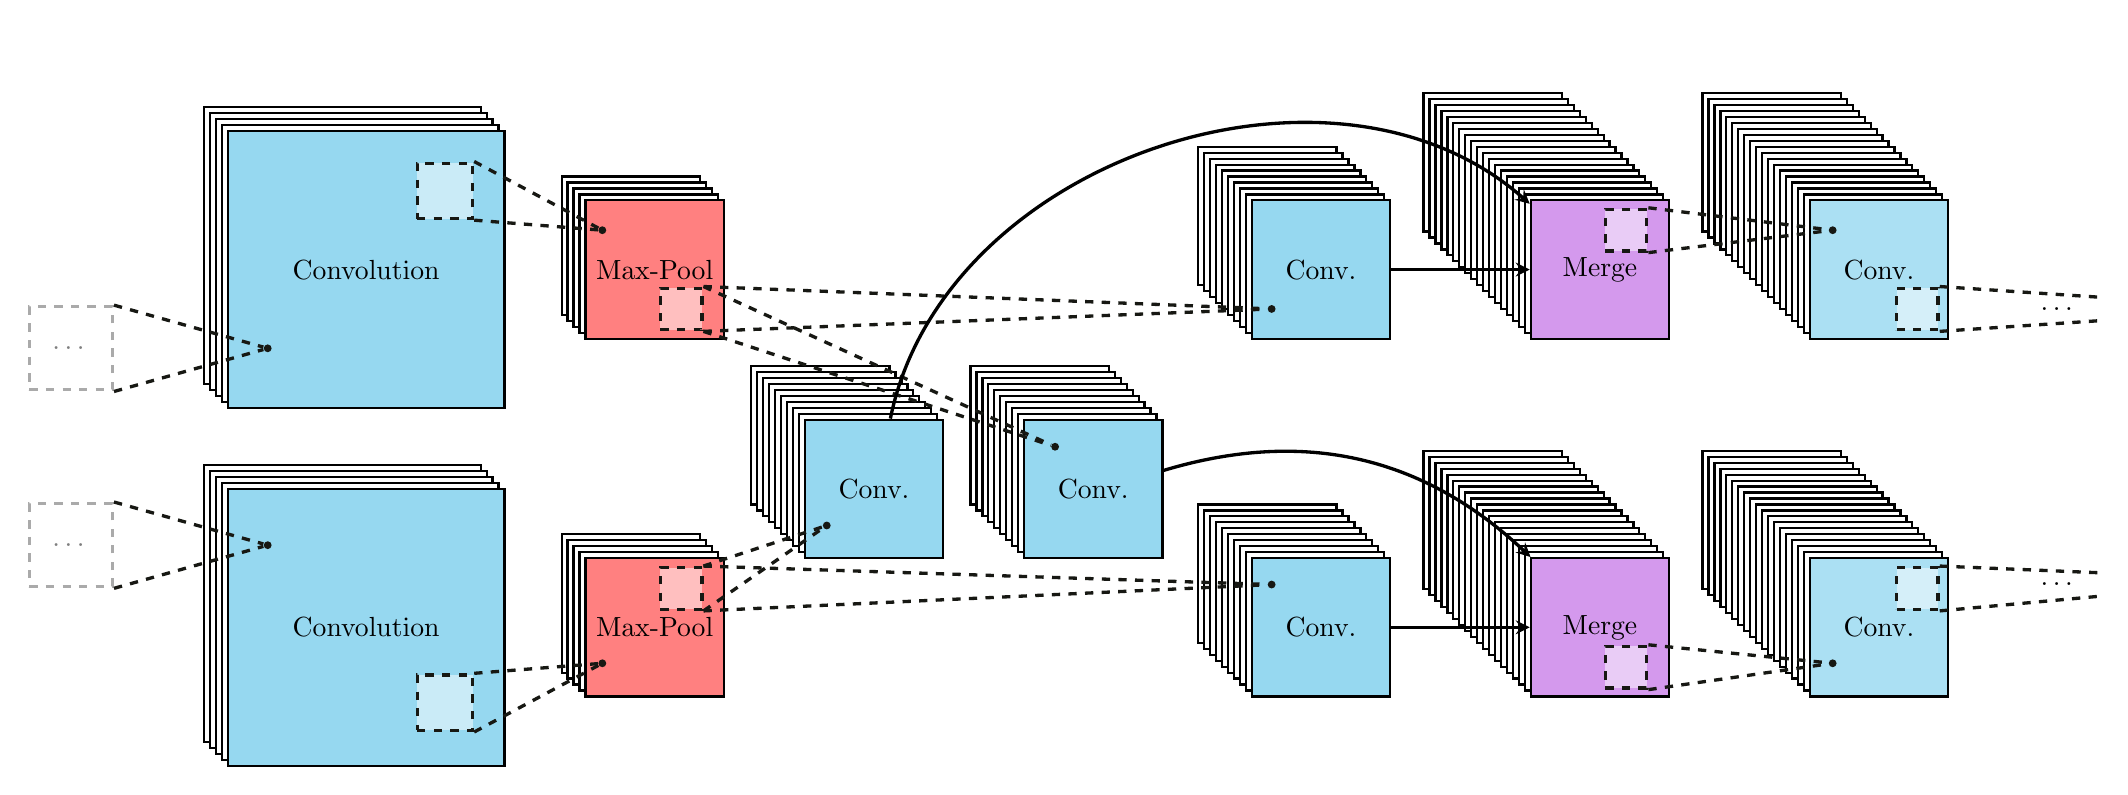
\begin{tikzpicture}
	
	\node [cascaded,
	fill = echoreg!50,
    minimum width = 10em,
    minimum height = 10em] (Conv1C) {Convolution};
	\node [cascaded,
	fill = echoreg!50,
    minimum width = 10em,
    minimum height = 10em,
	below= of Conv1C] (Conv1M) {Convolution};
    
    
	\node [cascaded,
	fill = red!50,
    minimum width = 5em,
    minimum height = 5em,right= of Conv1C] (Pool1C) {Max-Pool};
	\node [cascaded,
	fill = red!50,
    minimum width = 5em,
    minimum height = 5em,right= of Conv1M] (Pool1M) {Max-Pool};
    
    \node [cascadedd,
	fill = echoreg!50,
    minimum width = 5em,
    minimum height = 5em, below right= of Pool1C] (Conv2CM) {Conv.};
	\node [cascadedd,
	fill = echoreg!50,
    minimum width = 5em,
    minimum height = 5em,right= of Conv2CM] (Conv2MC) {Conv.};
    
    \node [cascadedd,
	fill = echoreg!50,
    minimum width = 5em,
    minimum height = 5em, right= 19em of Pool1C] (Conv3C) {Conv.};
	\node [cascadedd,
	fill = echoreg!50,
    minimum width = 5em,
    minimum height = 5em, right = 19em of Pool1M] (Conv3M) {Conv.};
    
    
    \node [cascadeddd,
	fill = mymauve!40,
    minimum width = 5em,
    minimum height = 5em, right= 5em of Conv3C] (Conv4C) {Merge};
	\node [cascadeddd,
	fill = mymauve!40,
    minimum width = 5em,
    minimum height = 5em, right = 5em of Conv3M] (Conv4M) {Merge};
    
     \node [cascadeddd,
	fill = echoreg!40,
    minimum width = 5em,
    minimum height = 5em, right=5em of Conv4C] (DeconvC) {Conv.};
    
	\node [cascadeddd,
	fill = echoreg!40,
    minimum width = 5em,
    minimum height = 5em, right =5em of Conv4M] (DeconvM) {Conv.};
    
    \node[rectangle, dashed, draw=lgry, fill=white,  fill opacity=0.5, very thick, minimum width=3em, minimum height=3em] (R1C) at (-3.75, -1) {\textcolor{black}{\dots}};
    
    \node[rectangle, dashed, draw=lgry, fill=white,  fill opacity=0.5, very thick, minimum width=3em, minimum height=3em] (R1M) at (-3.75, -3.5) {\textcolor{black}{\dots}};
    
    \node[rectangle, dashed, draw=sublimedg, fill=white,  fill opacity=0.5,very thick, minimum width=2em, minimum height=2em] (R2C) at (1, 1) {};
    
    \node[rectangle, dashed, draw=sublimedg, fill=white,  fill opacity=0.5,very thick, minimum width=2em, minimum height=2em] (R2M) at (1,-5.5) {};
    
    
    \node[rectangle, dashed, draw=sublimedg, fill=white,  fill opacity=0.5,very thick, minimum width=1.5em, minimum height=1.5em] (R3C) at (4, -0.5) {};
    
    \node[rectangle, dashed, draw=sublimedg, fill=white,  fill opacity=0.5,very thick, minimum width=1.5em, minimum height=1.5em] (R3M) at (4,-4.05) {};
    
    \node[rectangle, dashed, draw=sublimedg, fill=white,  fill opacity=0.5,very thick, minimum width=1.5em, minimum height=1.5em] (R4C) at (16, .5) {};
    
    \node[rectangle, dashed, draw=sublimedg, fill=white,  fill opacity=0.5,very thick, minimum width=1.5em, minimum height=1.5em] (R4M) at (16,-5.05) {};
    
    \node[rectangle, dashed, draw=sublimedg, fill=white,  fill opacity=0.5,very thick, minimum width=1.5em, minimum height=1.5em] (R5C) at (19.7, -.5) {};
    
    \node[rectangle, dashed, draw=sublimedg, fill=white,  fill opacity=0.5,very thick, minimum width=1.5em, minimum height=1.5em] (R5M) at (19.7, -4.05) {};
    
    \node[circle, inner sep = 0.1em, fill=sublimedg] (C1C) at (-1.25, -1) {};
    \node[circle, inner sep = 0.1em, fill=sublimedg] (C1M) at (-1.25, -3.5) {};
    
    \node[circle, inner sep = 0.1em, fill=sublimedg] (C2C) at (3, 0.5) {};
    \node[circle, inner sep = 0.1em, fill=sublimedg] (C2M) at (3, -5) {};
    
    \node[circle, inner sep = 0.1em, fill=sublimedg] (C3MC) at (5.85, -3.25) {};
    \node[circle, inner sep = 0.1em, fill=sublimedg] (C3CM) at (8.75, -2.25) {};
    
    \node[circle, inner sep = 0.1em, fill=sublimedg] (C4C) at (11.5, -0.5) {};
    \node[circle, inner sep = 0.1em, fill=sublimedg] (C4M) at (11.5, -4) {};
    
    \node[circle, inner sep = 0.1em, fill=sublimedg] (C5C) at (18.625, 0.5) {};
    \node[circle, inner sep = 0.1em, fill=sublimedg] (C5M) at (18.625, -5) {};
    
    \draw[very thick, sublimedg, dashed] (R1C.north east) -- (C1C);
    \draw[very thick, sublimedg, dashed] (R1C.south east) -- (C1C);
    \draw[very thick, sublimedg, dashed] (R1M.north east) -- (C1M);
    \draw[very thick, sublimedg, dashed] (R1M.south east) -- (C1M);
    
    \draw[very thick, sublimedg, dashed] (R2C.north east) -- (C2C);
    \draw[very thick, sublimedg, dashed] (R2C.south east) -- (C2C);
    \draw[very thick, sublimedg, dashed] (R2M.north east) -- (C2M);
    \draw[very thick, sublimedg, dashed] (R2M.south east) -- (C2M);
    
    \draw[very thick, sublimedg, dashed] (R3C.north east) -- (C3CM);
    \draw[very thick, sublimedg, dashed] (R3C.south east) -- (C3CM);
    \draw[very thick, sublimedg, dashed] (R3M.north east) -- (C3MC);
    \draw[very thick, sublimedg, dashed] (R3M.south east) -- (C3MC);
    
    \draw[very thick, sublimedg, dashed] (R3C.north east) -- (C4C);
    \draw[very thick, sublimedg, dashed] (R3C.south east) -- (C4C);
    \draw[very thick, sublimedg, dashed] (R3M.north east) -- (C4M);
    \draw[very thick, sublimedg, dashed] (R3M.south east) -- (C4M);
   
    \draw[very thick, sublimedg, dashed] (R4C.north east) -- (C5C);
    \draw[very thick, sublimedg, dashed] (R4C.south east) -- (C5C);
    \draw[very thick, sublimedg, dashed] (R4M.north east) -- (C5M);
    \draw[very thick, sublimedg, dashed] (R4M.south east) -- (C5M);
    
    \draw[very thick, sublimedg, dashed] (R5C.north east) -- (22, -0.35);
    \draw[very thick, sublimedg, dashed] (R5C.south east) -- (22, -0.65);
    \draw[very thick, sublimedg, dashed] (R5M.north east) -- (22, -3.85);
    \draw[very thick, sublimedg, dashed] (R5M.south east) -- (22, -4.15);
    
    \node[] (da) at (21.5, -0.5) {\textcolor{lgry}\bf\dots};
    \node[] (db) at (21.5, -4) {\textcolor{lgry}\bf\dots};
        
    \path[very thick, -stealth] (Conv2CM) edge[bend left=60] (Conv4C);
    \draw[very thick, -stealth] (Conv3C) -- (Conv4C);
    \path[very thick, -stealth] (Conv2MC) edge[bend left] (Conv4M);
    \draw[very thick, -stealth] (Conv3M) -- (Conv4M);
\end{tikzpicture}
\end{document}
